\documentclass[tikz,border=2pt]{standalone}
\usepackage{amsmath,amssymb}
\usetikzlibrary{arrows.meta}
\begin{document}
% Five-job single-server path: A = (0,1,2.5,6,7.5), S = (2,2,1,1,1.5), D = (2,4,5,7,9).
% L(t) (blue) and the values L(A_k-) = 0,1,1,0,0 seen by the arrivals (green dots):
% 3 of 5 arrivals see an empty system, although L = 0 for only 1.5 of the 9 minutes.
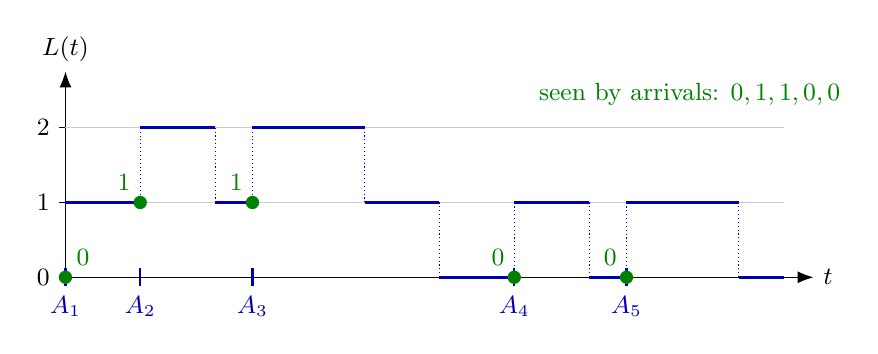
\begin{tikzpicture}[font=\small, >={Latex[length=2mm]}, x=0.95cm, y=0.95cm]
  % axes
  \draw[->] (0,0) -- (10,0) node[right] {$t$};
  \draw[->] (0,0) -- (0,2.75) node[above] {$L(t)$};
  \foreach \y in {1,2} {\draw (0.08,\y) -- (-0.08,\y) node[left] {$\y$};}
  \node[left] at (-0.08,0) {$0$};
  % grid lines for the levels
  \foreach \y in {1,2} {\draw[gray!40, thin] (0,\y) -- (9.6,\y);}
  % sample path (right-continuous steps)
  \draw[blue!70!black, very thick]
    (0,1) -- (1,1) (1,2) -- (2,2) (2,1) -- (2.5,1) (2.5,2) -- (4,2)
    (4,1) -- (5,1) (5,0) -- (6,0) (6,1) -- (7,1) (7,0) -- (7.5,0)
    (7.5,1) -- (9,1) (9,0) -- (9.6,0);
  \foreach \x/\a/\b in {1/1/2, 2/2/1, 2.5/1/2, 4/2/1, 5/1/0, 6/0/1, 7/1/0, 7.5/0/1, 9/1/0}
    {\draw[blue!70!black, thin, densely dotted] (\x,\a) -- (\x,\b);}
  % arrival epochs
  \foreach \x/\k in {0/1, 1/2, 2.5/3, 6/4, 7.5/5}
    {\draw[blue!70!black, thick] (\x,0.12) -- (\x,-0.12) node[below] {$A_{\k}$};}
  % what the arrivals see: L(A_k-)
  \foreach \x/\y in {0/0, 1/1, 2.5/1, 6/0, 7.5/0}
    {\fill[green!50!black] (\x,\y) circle (2.4pt);}
  \node[green!50!black, anchor=south east] at (1,1.03) {$1$};
  \node[green!50!black, anchor=south east] at (2.5,1.03) {$1$};
  \node[green!50!black, anchor=south west] at (0.02,0.03) {$0$};
  \node[green!50!black, anchor=south east] at (6,0.03) {$0$};
  \node[green!50!black, anchor=south east] at (7.5,0.03) {$0$};
  % summary
  \node[green!50!black, anchor=west, align=left] at (6.2,2.45) {seen by arrivals: $0,1,1,0,0$};
\end{tikzpicture}
\end{document}
